\documentclass[english, 12pt, a4paper, sci, utf8, a-2b, online]{aaltothesis}

%% DO NOT MOVE OR REMOVE \setupthesisfonts
\setupthesisfonts

%% Add here the packges you need
\usepackage{graphicx}

%% For tables that span multiple pages; used to split a paraphrasing example in
%% the appendix. If you don't need it, remove it.
\usepackage{longtable}

%% A package for generating Creative Commons copyright terms. If you don't use
%% the CC copyright terms, remove it, since otherwise undesired information may
%% be added to this document's metadata.
\usepackage[type={CC}, modifier={by-nc-sa}, version={4.0}]{doclicense}
%% Find below three examples for typesetting the CC license notice.

\degreeprogram{Computer, Communication and Information Sciences}
\major{Security and Cloud Computing}
\univdegree{MSc}
\thesisauthor{Oula Kivalo}

%% Your thesis title and possible subtitle comes here and possibly, again,
%% together with the Finnish or Swedish abstract. Do not hyphenate the title
%% (and subtitle), and avoid writing too long a title. Should LaTeX typeset a
%% long title (and/or subtitle) unsatisfactorily, you might have to force a
%% linebreak using the \\ control characters. In this case...
%% * Remember, the title should not be hyphenated!
%% * A possible 'and' in the title should not be the last word in the line; it
%%   begins the next line.
%% * Specify the title (and/or subtitle) again without the linebreak characters
%%   in the optional argument in box brackets. This is done because the title
%%   is part of the metadata in the pdf/a file, and the metadata cannot contain
%%   linebreaks.
%%
\thesistitle{Cross-language JSON parser interoperability}
%\thesistitle[Title of the thesis]{Title of\\ the thesis}

\place{Espoo}
\date{TODO}

%% Thesis supervisor
\supervisor{Prof.\ TODO}

%% Advisor(s)---two at the most---of the thesis. Check with your supervisor how
%% many official advisors you can have.
\advisor{TODO}
% \advisor{Dr Alan Advisor}
% \advisor{Ms Elsa Expert (MSc)}

%% Aaltologo: syntax:
%% \uselogo{?|!|'|aalto?|aalto!|aalto'|<empty>}
%% The logo language is set to be the same as the thesis language.
%%
%\uselogo{?}
%\uselogo{!}
\uselogo{'}
%\uselogo{aalto?}
%\uselogo{aalto!}
%\uselogo{aalto'}
%\uselogo{}
%%

%%%%%%%%%%%%%%%%%%               COPYRIGHT TEXT               %%%%%%%%%%%%%%%%%%
%%%%%%%%%%%%%%%%%%%%%%%%%%%%%%%%%%%%%%%%%%%%%%%%%%%%%%%%%%%%%%%%%%%%%%%%%%%%%%%%

%% Copyright of a work is with the creator/author of the work regardless of
%% whether the copyright mark is explicitly in the work or not. You may, if you
%% wish---we encourage you to do so---publish your work under a Creative
%% Commons license (see creativecommons.org), in which case the license text
%% must be visible in the work. Write here the copyright text you want using the
%% macro \copyrighttext, which writes the text into the metadata of the pdf file
%% as well.
%%
%% Syntax:
% \copyrigthtext{metadata text}{text visible on the page}
% \input{license.tex}
% \copyrigthtext{\license}{\license}
%%
%% CHOOSE ONE OF THE COPYRIGHT NOTICE STYLES BELOW.
%% IF USING THE CC TERMS, CHOOSE THE LICENSE YOU WANT TO USE.
%% The different CC licenses are listed at 
%% https://creativecommons.org/about/cclicenses/.
%% If you use the icons from the doclicense.sty package, add the package above
%% (\usepackage{doclicense}).
%% IMPORTANT NOTE!! Manually write the CC text in the \copyrighttext metadata
%% text field.
%%
%% NOTE: In the macros below, the text written in the metadata must have a
%% \noexpand macro before the \copyright special character. When not in pdf/a
%% mode (i.e. a-1b or a-2b are not specified in \documentclass), two \noexpands
%% are required in the metadata text to correctly render the copyright mark in
%% the pdf metadata. In pdf/a mode one \noexpand suffices.
%%
%% EXAMPLE OF PLAIN COPYRIGHT TEXT
%% The macros \copyright and \year below must be separated by the \ character 
%% (space chacter) from the text that follows. The macros in the argument of the
%% \copyrighttext macro automatically insert the year and the author's name.
%% (Note! \ThesisAuthor is an internal macro of the aaltothesis.cls class file).
%%
%\copyrighttext{Copyright \noexpand\textcopyright\ \number\year\ \ThesisAuthor}
%{Copyright \textcopyright{} \number\year{} \ThesisAuthor}
%%
%% Of course, the same text could have simply been written as
%% \copyrighttext{Copyright \noexpand\copyright\ 2018 Eddie Engineer}
%% {Copyright \copyright{} 2022 Eddie Engineer}
%%
%% EXAMPLES OF CC LICENSE: different ways to display the same license
%% 1. A simple Creative Commons license text with a link to the copyright notice:
%\copyrighttext{\noexpand\textcopyright\ \number\year. This work is 
%	licensed under a CC BY-NC-SA 4.0 license.}{\textcopyright{} 
%	\number\year. This work is licensed under a 
%	\href{https://creativecommons.org/licenses/by-nc-nd/4.0/}{CC BY-NC-SA 4.0} 
%	license.}
%
%% To get the URL of the license of your choice, go to 
%% https://creativecommons.org/about/cclicenses/, click on the chosen license
%% you want to use, and copy-and-paste the URL in the macro \href above.
%%
%% 2. A short Creative Commons license text containing the respective CC icons
%% (requires the package doclicense.sty to be added in the preamble as done
%% above) and a link to the corresponding Creative Commons license webpage (see
%% the doclicense package documentation for other license icons):
%\copyrighttext{\noexpand\textcopyright\ \number\year. This work is licensed
%	under a CC BY-NC-SA 4.0 license.}{
%	\parbox{95mm}{\noindent\textcopyright\ \number\year. \doclicenseText} 
%	\hspace{1em}\parbox{35mm}{\doclicenseImage}
%}
%%
%% 3. An expanded Creative Commons license text containing the respective CC
%% icons text and as generated by the doclicense.sty package (the license is set
%% via package options in \usepackage[options]{doclicense} above; see the
%% doclicense package documentation for other license texts and icons):
\copyrighttext{\noexpand\textcopyright\ \number\year. This work is 
	licensed under a Creative Commons "Attribution-NonCommercial-ShareAlike 4.0 
	International" (BY-NC-SA 4.0) license.}{\noindent\textcopyright\ \number
	\year \ \doclicenseThis}
%%%%%%%%%%%%%%%%%%%%%%%%%%%%%%%%%%%%%%%%%%%%%%%%%%%%%%%%%%%%%%%%%%%%%%%%%%%%%%%%


%% The English abstract:
%% All the details (name, title, etc.) on the abstract page appear as specified
%% above.
%% Thesis keywords:
%% Note! The keywords are separated using the \spc macro
%%
% \keywords{For keywords choose\spc concepts that are\spc central to your\spc 
% thesis}
\keywords{JSON parsing\spc JSON interoperability\spc Cross-language parsing}
%%

%% The abstract text. This text in one paragraph is included in the metadata of
%% the pdf file as well as the abstract page. To have paragraphs in your
%% abstract rewrite it in the abstarct environment as described below.
%%

\thesisabstract{TODO}

%% You can prevent LaTeX from writing into the xmpdata file (it contains all the 
%% metadata to be written into the pdf file) by setting the writexmpdata switch
%% to 'false'. This allows you to write the metadata in the correct format
%% directly into the file thesistemplate.xmpdata.
%\setboolean{writexmpdatafile}{false}

\def\note#1{\begin{flushleft}
	{\color{orange} \raggedright \textsf{#1}}
 \linebreak \noindent
\end{flushleft}}

\def\str#1{\texttt{'#1'}}

%% All that is printed on paper starts here
%%
\begin{document}

%% Create the coverpage
%%
\makecoverpage

%% Typeset the copyright text.
%% If you wish, you may leave out the copyright text from the human-readable
%% page of the pdf file. This may seem like a attractive idea for the printed
%% document especially if "Copyright (c) yyyy Eddie Engineer" is the only text
%% on the page. However, the recommendation is to print this copyright text.
%%
\makecopyrightpage

\clearpage
%% Note that when writing your thesis in English, place the English abstract
%% first followed by the possible Finnish or Swedish abstract.

%% Abstract text
%% All the details (name, title, etc.) on the abstract page appear as specified
%% above. Add your abstarct text with paragraphs here to have paragraphs in the
%% visible abstract page. Nonetheless, write the abstarct text without
%% paragraphs in the macro \thesismacro so that it is added to the metadata as
%% well.
%%
\begin{abstractpage}[english]
	TODO
  % The abstract is a short description of the essential contents of the thesis,
  % usually in one paragraph: what was studied and how and what were the main
  % findings.
  %
  % For a Finnish thesis, the abstract should be written in both Finnish and
  % English; for a Swedish thesis, in Swedish and English. The abstracts for
  % English theses written by Finnish or Swedish speakers should be written in
  % English and either in Finnish or in Swedish, depending on the student’s
  % language of basic education. Students educated in languages other than Finnish
  % or Swedish write the abstract only in English. Students may include a second
  % or third abstract in their native language, if they wish.
  %
  % The abstract text of this thesis is written on the readable abstract page as
  % well as into the pdf file's metadata via the \verb+\thesisabstract+ macro
  % (see comment in this \TeX{} file above). Write here the text that goes onto
  % the readable abstract page. You can have special characters, linebreaks, and
  % paragraphs here. Otherwise, this abstract text must be identical to the
  % metadata abstract text.
  %
  % If your abstract does not contain special characters and it does not require
  % paragraphs, you may take advantage of the \verb+\abstracttext+ macro (see the
  % comment in this \TeX{} file below).

%% The text in the \thesisabstract macro is stored in the macro \abstractext, so
%% you can use the text metadata abstract directly as follows:
%%
%\begin{abstractpage}[english]
%	\abstracttext{}
%\end{abstractpage}

%% Force a new page so that the possible Finnish or Swedish abstract does not
%% begin on the same page
%%
% \newpage
%%
%% Abstract in Finnish. Delete if you don't need it. 
%%
%% Respecify those fields that differ from the earlier specification or simply
%% respecify all fields.
% TODO - Tiivistelmä suomeksi
% \thesistitle{Opinnäyteen otsikko}
% \thesissubtitle{Opinnäytteen mahdollinen alaotsikko}
% \supervisor{Prof.\ Pirjo Professori}
% \advisor{TkT Alan Advisor}
% \advisor{DI Elsa Expert}
% \degreeprogram{Elektroniikka ja sähkötekniikka}
% \major{Sopiva pääaine}
% \collaborativepartner{Yhtiön tai laitoksen nimi (tarvittaessa)}
% \date{30.6.2025}
% %% The keywords need not be separated by \spc now.
% \keywords{Vastus, resistanssi, lämpötila}
% %% Abstract text
% \begin{abstractpage}[finnish]
% Tiivistelmä on lyhyt kuvaus työn keskeisestä sisällöstä usein yhtenä kappaleena:
% mitä tutkittiin ja miten sekä mitkä olivat tärkeimmät tulokset. Suomenkielisen
% opinnäytteen tiivistelmä kirjoitetaan suomeksi ja englanniksi ja ruotsinkielisen
% vastaavasti ruotsiksi ja englanniksi. Suomen- tai ruotsinkielisten
% opiskelijoiden, joiden opinnäytteen kieli on englanti, tulee kirjoittaa
% tiivistelmänsä englanniksi ja koulusivistyskielellään. Muiden kuin
% koulusivistyskieleltään suomen- tai ruotsinkielisten tulee kirjoittaa
% tiivistelmänsä vain englanniksi. Opiskelija voi halutessaan lisätä
% opinnäytteeseensä toisen tai kolmannen tiivistelmän omalla äidinkielellään.
% Tämän opinnäytteen tiivistelmäteksti kirjoitetaan opinnäytteen luettavan osan
% lomakkeen lisäksi myös pdf-tiedoston metadataan. Kirjoita tähän metadataan
% kirjoitettavaa teksti. Metadatatekstissa ei saa olla erikoismerkkejä,
% rivinvaiho- tai kappaleenjakomerkkiä, joten näitä merkkeja ei saa käyttää tässä.
% Jos tiivistelmäsi ei sisällä erikoimerkkejä eikä kaipaa kappaleenjakoa, voit
% hyödynttää makroa abstracttext luodessasi lomakkeen tiivistelmää (katso
% kommentti tässä TeX-tiedostossa alla). Metadatatiivistelmatekstin on muuten 
% oltava sama kuin lomakkeessa oleva teksti.
%
% \end{abstractpage}
\end{abstractpage}

%% Force new page so that the Swedish abstract starts from a new page

%% Preface
%%
%% This section is optional. Remove it if you do not want a preface.
% \mysection{Preface}
% %\mysection{Esipuhe}
% I want to thank Professor Pirjo Professor and my instructors Dr Alan Advisor and
% Ms Elsa Expert for their guidance.
%
% I also want to thank my partner for keeping me sane and alive.
%
% \vspace{5cm}
% Otaniemi, 30 June 2025\\
%
% \vspace{5mm}
% {\hfill Eddie E.\ Engineer \hspace{1cm}}
%
% %% Force a new page after the preface
% %%
% \newpage


%% Table of contents.
\newpage
\thesistableofcontents


%% Symbols and abbreviations
\mysection{Symbols and abbreviations}
\subsection*{Symbols}

\begin{tabular}{ll}
	$P$		& set of parsers \\
	$S$		& set of parsing results
	% $\mathbf{B}$  & magnetic flux density  \\
	% $c$              & speed of light in vacuum $\approx 3\times10^8$ [m/s]\\
	% $\omega_{\mathrm{D}}$    & Debye frequency \\
	% $\omega_{\mathrm{latt}}$ & average phonon frequency of lattice \\
	% $\uparrow$       & electron spin direction up\\
	% $\downarrow$     & electron spin direction down
\end{tabular}

% \subsection*{Operators}
%
% \begin{tabular}{ll}
% 	$\nabla \times \mathbf{A}$              & curl of vectorin $\mathbf{A}$\\
% 	$\displaystyle\frac{\mbox{d}}{\mbox{d} t}$ & derivative with respect to 
% 	variable $t$\\[3mm]
% 	$\displaystyle\frac{\partial}{\partial t}$  & partial derivative with respect 
% 	to variable $t$ \\[3mm]
% 	$\sum_i $                       & sum over index $i$\\
% 	$\mathbf{A} \cdot \mathbf{B}$    & dot product of vectors $\mathbf{A}$ and 
% 	$\mathbf{B}$
% \end{tabular}

\subsection*{Abbreviations}

\begin{tabular}{ll}
	JSON	& JavaScript object notation \\
	IETF	& internet engineering task force \\
	RLE		& Run-length encoding
% AC         & alternating current \\
% APLAC      & an object-oriented analog circuit simulator and design tool \\
%            & (originally Analysis Program for Linear Active Circuits) \\
% BCS        & Bardeen-Cooper-Schrieffer \\ %% dash between the names
% DC         & direct current \\
% TEM        & transverse eletromagnetic
\end{tabular}


\subsection*{Strings}
\note{TODO - Not sure where to place this}
Unless otherwise specified, strings in this paper represent a character sequence encoded in UTF-8. Strings are surrounded by single quotation marks "\texttt{'}" which are not included in them. Example: \str{\{"key": "value"\}}.

There are a few character sequences which have a special meaning and are encoded following different rules:

\vspace{8pt}

\begin{tabular}{lll}
	Sequence & Description & Encoding \\
	\hline
	$\texttt{\textbackslash n}$ & New line character & $\texttt{0A}$ in hexadecimal \\
	$\texttt{\textbackslash t}$ & Horizontal tab & $\texttt{09}$ in hexadecimal \\
	$\texttt{\textbackslash r}$ & Carriage return & $\texttt{0D}$ in hexadecimal \\
	$\texttt{\textbackslash x}a$ & Single byte. & Single byte with a \\
	 & $a$ is as a two digit hexadecimal number & value of $a$  \\
	 & with a range of $a \in \{0, 1, ..., 255\}$ & 
	% $$ & Encoded as a single byte placed between & $$ \\
	% $$ & its surrounding characters & $$ \\
	% $$ & in UTF-8. May be used to produce invalid UTF-8 strings. & $$
\end{tabular}



%% \clearpage is similar to \newpage, but it also flushes the floats (figures
%% and tables).
%%
\cleardoublepage

%% Text body begins.
%%
\section{Introduction}
% \label{sec:intro}
\note{\emph{Comments are colored in orange.} \\
This thesis is currently in its initial stages and will be rewritten. As such, I'm looking for feedback on its general structure, and not on its text. \\
This chapter is mostly copied from the thesis proposal}

JavaScript Object Notation(JSON) has become the de facto standard for data interchange on the internet, and as such, multiple parsers have been developed for it across programming languages. With the rise of microservice-based cloud architectures, where small independent services often utilize JSON for communication, these different parser implementations may be used to parse the same inputs. If a malicious actor is able to inject JSON data into such communication, inconsistencies in parser behavior may enable privilege escalation, denial-of-service attacks, or other vulnerabilities.

Even with its minimalistic design, JSON parsing can introduce security vulnerabilities due to ambiguities in the specification and incorrect parser implementations. Due to its apparent simplicity and minimalistic featureset, JSON can easily be missed as a potential attack vector.


\subsection{Problem statement}
Despite the widespread use of JSON, academic research on JSON parser interoperability is surprisingly limited. Most prior work has been carried out by independent security researchers, though their findings are already several years old and may be outdated. This thesis aims to further research in the area by documenting interoperability concerns across different parser implementations in multiple programming languages.

This thesis builds on the work of Möller et al., who showed that JSON parsers have large amounts of discrepancies between them. This is done by investigating a larger set of parsers and placing a focus on major discrepancies between them which may lead to vulnerabilities.

This thesis tests a collection of 40 parsers across ten languages.

\note{TODO - update parser count}


\subsection{Structure of the thesis}
\note{TODO}

%% Leave page number of the first page empty
\thispagestyle{empty}

% \subsection{Typical content in the introduction}
%
% In principle, the introduction is like the abstract, only broader in scope, and
% more detailed. The introduction generally describes the following:
%
% %% An example of an unordered (itemised) list. Instead on the default bullet
% %% point, an endash (-- in LaTeX code) is used as the item label.
% \begin{itemize}
% 	\item[--] a description of the background of the field of study, what
% 	similar work others have already done, as well as an overview of the study,
% 	\item[--] the goals of the study,
% 	\item[--] the primary research question and the sub-problems in the line
% 	of inquiry, and
% 	\item[--] the scope and constraints of the study along with the main
% 	concepts involved.
% \end{itemize}
%
% Although the introduction is a general description of the study, be concise and 
% avoid writing a lengthy introduction. A concise introduction need not have any 
% subsections.

%% In a thesis, every section/chapter starts a new page, hence the \clearpage
\clearpage
\section{Background}


\subsection{JavaScript object notation}
\note{TODO - Introduction to JSON and its specification}


\subsubsection{History of JSON}
\note{TODO - Brief overview of how we got here. Historical baggage in JSON}


\subsubsection{Ambiguities in the JSON specification}
\begin{itemize}
	\item Duplicate key precedence
	\item Character encoding% (\textbackslash uXXXX form, UTF-16 surrogate bytes)
	\item String comparison
	\item Extremely large numbers
	\item Nesting depth
	\item Version numbering, or lack thereof
\end{itemize}


\subsection{Fuzz testing}
\note{TODO - What fuzz testing is and what can be achieved using it.}


\subsubsection{Mutation based fuzz testing}
\note{TODO - Mutating hand-picked test cases in different ways.}

% \subsubsection{Coverage based fuzz testing \emph{(Most likely out of scope)}}
% \note{TODO - Generating test cases based on what sections of the tested code are being executed.}


\subsubsection{Black-box fuzzing}
\note{Not sure whether automatic test case generation will be implemented. I have some plans on how I could implement this for black-box fuzzing, but this might be out of scope for the thesis}


\subsubsection{Cross-language fuzz testing}
\note{TODO - Testing something across multiple programming languages and seeing how results differ with the same test case.}

% \subsubsection{Reverse proxy}
% \note{TODO - Testing something across multiple programming languages and seeing how results differ with the same test case.}


\subsubsection{Previous work in JSON fuzz testing}
Current fuzz testing is mostly focused on individual parsers and rarely includes other parsers. Popular parsers commonly have a test suite which contains edge cases and fuzz testing.


\subsection{Run-length encoding}
Run-length encoding (RLE) is a lossless form of data compression where consecutive identical occurences of data are stored as a single occurence of the data and a count of its consecutive occurences. It has an extremely low overhead and provides good compression ratios for data which contains repeated values often.


\subsection{Vulnerabilities}
\note{Will be updated depending on findings and related work}
\subsubsection{Denial of service}
\subsubsection{Remote code execution}


\clearpage
\section{Methods}


\subsection{Parser selection}
The parsers were selected from \url{json.org} and GitHub based on their popularity.


\subsection{Testing parsers}
Parsers were tested using a custom fuzzing application.


\subsection{Test case selection}
Test cases used for mutation-based fuzz testing were selected from edge cases shown in the JSON specification and from the test suites of popular parsers.


\subsection{Analyzing results}
The results gained from fuzzing were stored for later analyzis.


\subsection{Searching vulnerabilities}
Using the results gained from fuzzing, open source projects were investigated for potential vulnerabilities.


\clearpage

\section{Implementation}
\subsection{Tooling}
Due to the large number of dependencies used, everything was implemented inside a Docker container running in a Linux environment. The programs developed for the thesis were written in multiple different programming languages:

\begin{enumerate}
	\item Bash
	\item C++
	\item Clojure
	\item Golang
	\item JavaScript
	\item Lua
	\item PHP
	\item Python
	\item Rust
\end{enumerate}

The fuzzer and analyzer were written in Rust due to the large amounts of data processed. The project uses multiple helper scripts written in Bash. Other languages used were needed for the JSON parsers.


\subsubsection{Libraries used}
\note{TODO - an ungodly amount. Need to condense this section to fit within the page target count for a master's thesis. I also refer to different JSON parsers by a custom codename. Need to put a list of them here}


\subsection{Test server}
\note{TODO - Discuss fuzzing implementation}
Test server generates test cases and shares them with clients via TCP sockets. Due to the high performance requirements, the server was written using Rust.


\subsection{Clients}
Clients contain multiple JSON parsers which parse the incoming data sent by the test server. Each JSON parser has their own client instance which connects to the test server.

Some clients support multiple languages. The client for C++ also contains parsers for C. The client for Clojure also contains parsers for Java.


\subsection{Server-client communication}
A custom binary protocol over TCP was developed for the thesis.


\subsection{Result compression and decompression}
The server saved the parsing results for later analysis. Due to the total size of the parsing results being over a petabyte, an efficient compression solution was needed. After existing solutions were tested and their performance was deemed unsatisfactory, a custom solution based on run-length encoding (RLE) was developed.

The set of parsing results $S$ contains the following elements:

\begin{equation}
	S \in \{(p, d, r) \mid p \in P, d,r \in \{0,1\}^*\}
\end{equation}

where $P$ is the set of parsers, $d$ is binary representation of JSON data, and $r$ is the parsing result parser $p$ produced for input $d$.

\note{TODO - Explain how most of this information can be stripped during compression, run-length encoding (RLE), the binary data format used, and how it can be decompressed.}


\subsection{Analysis}

% \begin{equation}
% 	S = \{(p, d, r) \mid p \in P, d,r \in \{0,1\}*\}
% \end{equation}
%
% ${(c, d, r) \mid c_{0} \ne c_{1}, }$
% ${(c_{0}, c_{1}, d, r) \mid c_{0} \ne c_{1}, }$


\clearpage

\section{Results}
\subsection{JSON parsing inconsistencies}
\subsubsection{Different value access in JSON objects}
\note{TODO - Main contribution}
JSON parsers can retrieve different values from the same object when querying for the same key as seen in Figure \ref{fig:mismatches} and table \ref{appendix:mismatches}.

% \begin{figure}[tb]
\begin{figure}
  \centering
  % 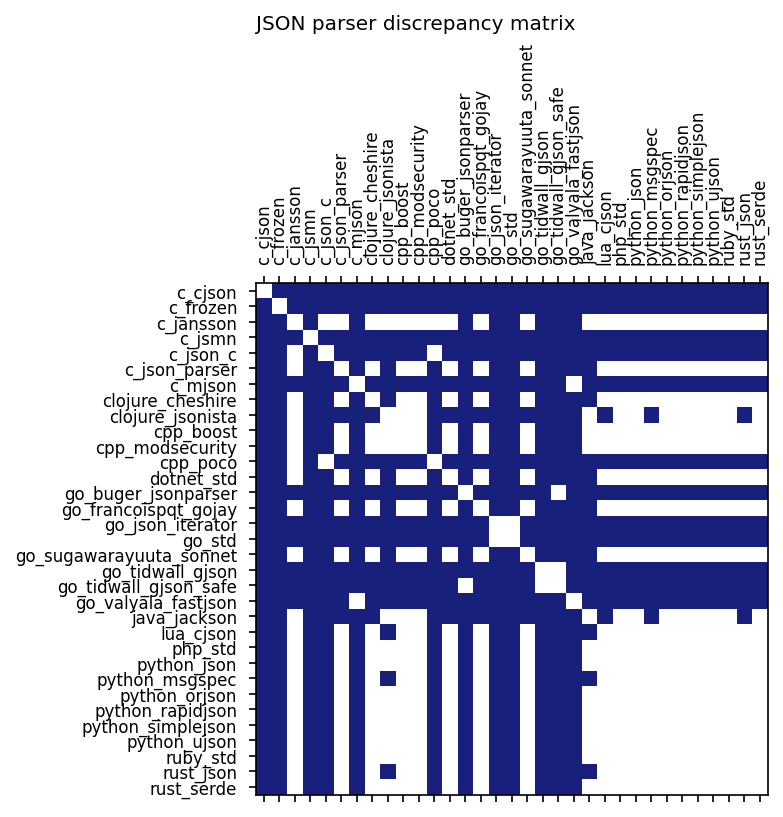
\includegraphics[alt={JSON parsing inconsistencies}, height=5cm]{./figures/parsing_mismatches.png}
  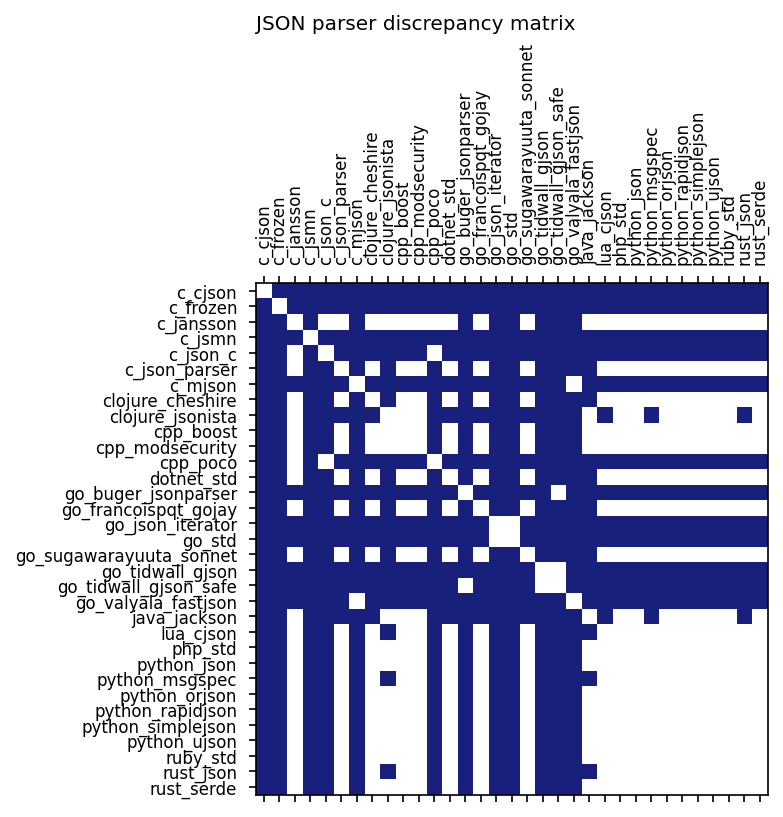
\includegraphics[alt={JSON parsing inconsistencies}]{./figures/parsing_mismatches.png}
  \caption{JSON parsing mismatches. A cell is colored in blue if the parsers in the corresponding column and row can retrieve different values when querying the same key in the same JSON object.}
  \label{fig:mismatches}
\end{figure}


\subsection{Impact}
% \note{TODO - Search for vulnerabilities in open source projects based on the results gained.}


\subsubsection{Schema bypass in Tyk}
\note{Copied from gitlab with slight modifications}
Tyk is an API gateway which can be used to access multiple internal API's through a single external access point. It can be configured from a single OpenAPI document which provides information on how an API is structured and how it can be interacted with. Additionally, Tyk can be used to validate requests and responses going through it based on schemas defined in the OpenAPI document.

Hypothetical scenario
A login API is accessible thgough Tyk as shown in Figure 1. Tyk validates login information using JSON schemas contained in an OpenAPI document. In this scenario, the API developer believes the login information to be validated and passes it unsafely to an SQL query.
Due to Golang standard library JSON parser being case-insensitive, the schema validation can be bypassed by passing additional capitalized key-value pairs to the API.


\subsubsection{Rate limiting bypass in HAProxy}
\note{Copied from gitlab with slight modifications}
HAProxy is a popular reverse proxy with over a billion downloads in Docker Hub described as "a free, very fast and reliable reverse-proxy offering high availability, load balancing, and proxying for TCP and HTTP-based applications". One of its features is to act as a rate limiter between a client and a server. As an example, it can be configured to rate-limit requests by dropping those that match a certain IP address, header, URL, or body parameter after too many have been received within a timespan.

Internally, HAProxy uses mjson to parse JSON data inside request bodies and headers. When encountering duplicate keys, mjson uses only the first duplicate key while ignoring the rest. While this functionality is correct according to the latest JSON specification, it differs from the industry standard of using the last duplicate key inside JSON objects. Additionally, msjon does not parse unicode encoded values in strings.

Due to these discrepancies, the JSON object \\
\str{\{"rol\textbackslash u0065":"admin","role":"user","role":"admin"\}} gets parsed differently by mjson and the vast majority of other JSON parsers. While msjon believes that the key role has a value of user, almost all other parsers believe the value to be admin. This enables us to affect how HAProxy routes traffic when it is dependent on JSON values.

Hypothetical scenario
An API is behind HAProxy, which combines multiple different API's to a single externally accessible endpoint. One of these API's handles user logins. To prevent password guessing and brute forcing, HAProxy limits the number of login attempts for a single username from the same IP address. If the number of login attempts exceeds five within a 60 second window, the proxy denies additional 
%requests with HTTP status code 429: HTTP_TOO_MANY_REQUESTS.

Due to the API only accepting JSON data inside the POST request, HAProxy gets the username used for the rate limiting from JSON data.
Using the discrepancies described above, we can formulate the login request as \\ \str{\{"usernam\textbackslash u0065":"<actual>", "username":"<haproxy>",\\ "username":"<actual>", "password":"<password>"\}}. In this way, HAProxy and the API disagree on what the requested username is. Thus we can bypass the rate limiting by sending random information in the second field, while sending the actual username in the first and third fields.

\clearpage


\section{Evaluation}
\subsection{Limitations}
\subsection{Results}



\section{Conclusions}

\clearpage

%% Bibliography/ list of references
\thesisbibliography

\begin{thebibliography}{99}
		TODO
\end{thebibliography}



\clearpage

\thesisappendix

\section{JSON parsing mismatches}
\label{appendix:mismatches}

\scriptsize
\begin{longtable}{lllll}
    P1 & P2 & JSON & P1["q"] & P2["q"] \\
    \hline \\
    c\_cjson & c\_jansson & \str{\{"q":2,"q":3\}} & \str{2} & \str{3} \\
    c\_cjson & c\_json\_parser & \str{\{"q":2,"q":3\}} & \str{2} & \str{3} \\
    c\_cjson & c\_mjson & \str{\{"\textbackslash u0071":2,"q":3\}} & \str{2} & \str{3} \\
    c\_cjson & clojure\_cheshire & \str{\{"q":2,"q":3\}} & \str{2} & \str{3} \\
    c\_cjson & clojure\_jsonista & \str{\{"q":2,"q":3\}} & \str{2} & \str{3} \\
    c\_cjson & cpp\_modsecurity & \str{\{"q":2,"q":3\}} & \str{2} & \str{3} \\
    c\_cjson & go\_buger\_jsonparser & \str{\{"q\textbackslash u0000":2,"q":3\}} & \str{2} & \str{3} \\
    c\_cjson & go\_francoispqt\_gojay & \str{\{"q":2,"q":3\}} & \str{2} & \str{3} \\
    c\_cjson & go\_json\_iterator & \str{\{"q":2,"q":3\}} & \str{2} & \str{3} \\
    c\_cjson & go\_std & \str{\{"q":2,"q":3\}} & \str{2} & \str{3} \\
    c\_cjson & go\_sugawarayuuta\_sonnet & \str{\{"q":2,"q":3\}} & \str{2} & \str{3} \\
    c\_cjson & go\_tidwall\_gjson & \str{\{"q\textbackslash u0000":2,"q":3\}} & \str{2} & \str{3} \\
    c\_cjson & go\_tidwall\_gjson\_safe & \str{\{"q\textbackslash u0000":2,"q":3\}} & \str{2} & \str{3} \\
    c\_cjson & go\_valyala\_fastjson & \str{\{"\textbackslash u0071":2,"q":3\}} & \str{2} & \str{3} \\
    c\_cjson & java\_jackson & \str{\{"q":2,"q":3\}} & \str{2} & \str{3} \\
    c\_cjson & lua\_cjson & \str{\{"q":2,"q":3\}} & \str{2} & \str{3} \\
    c\_cjson & php\_std & \str{\{"q":2,"q":3\}} & \str{2} & \str{3} \\
    c\_cjson & python\_json & \str{\{"q":2,"q":3\}} & \str{2} & \str{3} \\
    c\_cjson & python\_msgspec & \str{\{"q":2,"q":3\}} & \str{2} & \str{3} \\
    c\_cjson & python\_orjson & \str{\{"q":2,"q":3\}} & \str{2} & \str{3} \\
    c\_cjson & python\_rapidjson & \str{\{"q":2,"q":3\}} & \str{2} & \str{3} \\
    c\_cjson & python\_simplejson & \str{\{"q":2,"q":3\}} & \str{2} & \str{3} \\
    c\_cjson & python\_ujson & \str{\{"q":2,"q":3\}} & \str{2} & \str{3} \\
    c\_cjson & rust\_json & \str{\{"q":2,"q":3\}} & \str{2} & \str{3} \\
    c\_cjson & rust\_serde & \str{\{"q":2,"q":3\}} & \str{2} & \str{3} \\
    c\_jansson & c\_cjson & \str{\{"q":2,"q":3\}} & \str{2} & \str{3} \\
    c\_jansson & c\_mjson & \str{\{"q":3,"q":2\}} & \str{2} & \str{3} \\
    c\_jansson & go\_buger\_jsonparser & \str{\{"q":3,"q":2\}} & \str{2} & \str{3} \\
    c\_jansson & go\_json\_iterator & \str{\{"q":2,"Q":3\}} & \str{2} & \str{3} \\
    c\_jansson & go\_std & \str{\{"q":2,"Q":3\}} & \str{2} & \str{3} \\
    c\_jansson & go\_tidwall\_gjson & \str{\{"q":3,"q":2\}} & \str{2} & \str{3} \\
    c\_jansson & go\_tidwall\_gjson\_safe & \str{\{"q":3,"q":2\}} & \str{2} & \str{3} \\
    c\_jansson & go\_valyala\_fastjson & \str{\{"q":3,"q":2\}} & \str{2} & \str{3} \\
    c\_json\_parser & c\_cjson & \str{\{"q":2,"q":3\}} & \str{2} & \str{3} \\
    c\_json\_parser & c\_mjson & \str{\{"q":3,"q":2\}} & \str{2} & \str{3} \\
    c\_json\_parser & clojure\_jsonista & \str{\{"q":2,"\textbackslash xffq":3\}} & \str{2} & \str{3} \\
    c\_json\_parser & go\_buger\_jsonparser & \str{\{"q":3,"q":2\}} & \str{2} & \str{3} \\
    c\_json\_parser & go\_json\_iterator & \str{\{"q":2,"Q":3\}} & \str{2} & \str{3} \\
    c\_json\_parser & go\_std & \str{\{"q":2,"Q":3\}} & \str{2} & \str{3} \\
    c\_json\_parser & go\_tidwall\_gjson & \str{\{"q":3,"q":2\}} & \str{2} & \str{3} \\
    c\_json\_parser & go\_tidwall\_gjson\_safe & \str{\{"q":3,"q":2\}} & \str{2} & \str{3} \\
    c\_json\_parser & go\_valyala\_fastjson & \str{\{"q":3,"q":2\}} & \str{2} & \str{3} \\
    c\_json\_parser & java\_jackson & \str{\{"q":2,"\textbackslash xffq":3\}} & \str{2} & \str{3} \\
    c\_mjson & c\_cjson & \str{\{"\textbackslash u0071":2,"q":3\}} & \str{2} & \str{3} \\
    c\_mjson & c\_jansson & \str{\{"q":3,"q":2\}} & \str{2} & \str{3} \\
    c\_mjson & c\_json\_parser & \str{\{"q":3,"q":2\}} & \str{2} & \str{3} \\
    c\_mjson & clojure\_cheshire & \str{\{"q":2,"q":3\}} & \str{2} & \str{3} \\
    c\_mjson & clojure\_jsonista & \str{\{"q":2,"q":3\}} & \str{2} & \str{3} \\
    c\_mjson & cpp\_modsecurity & \str{\{"q":2,"q":3\}} & \str{2} & \str{3} \\
    c\_mjson & go\_buger\_jsonparser & \str{\{"\textbackslash u0071":2,"q":3\}} & \str{3} & \str{2} \\
    c\_mjson & go\_francoispqt\_gojay & \str{\{"q":2,"q":3\}} & \str{2} & \str{3} \\
    c\_mjson & go\_json\_iterator & \str{\{"q":2,"q":3\}} & \str{2} & \str{3} \\
    c\_mjson & go\_std & \str{\{"q":2,"q":3\}} & \str{2} & \str{3} \\
    c\_mjson & go\_sugawarayuuta\_sonnet & \str{\{"q":2,"q":3\}} & \str{2} & \str{3} \\
    c\_mjson & go\_tidwall\_gjson & \str{\{"q\textbackslash q":2,"q":3\}} & \str{3} & \str{2} \\
    c\_mjson & go\_tidwall\_gjson\_safe & \str{\{"\textbackslash u0071":2,"q":3\}} & \str{3} & \str{2} \\
    c\_mjson & java\_jackson & \str{\{"q":2,"q":3\}} & \str{2} & \str{3} \\
    c\_mjson & lua\_cjson & \str{\{"q":2,"q":3\}} & \str{2} & \str{3} \\
    c\_mjson & php\_std & \str{\{"q":2,"q":3\}} & \str{2} & \str{3} \\
    c\_mjson & python\_json & \str{\{"q":2,"q":3\}} & \str{2} & \str{3} \\
    c\_mjson & python\_msgspec & \str{\{"q":2,"q":3\}} & \str{2} & \str{3} \\
    c\_mjson & python\_orjson & \str{\{"q":2,"q":3\}} & \str{2} & \str{3} \\
    c\_mjson & python\_rapidjson & \str{\{"q":2,"q":3\}} & \str{2} & \str{3} \\
    c\_mjson & python\_simplejson & \str{\{"q":2,"q":3\}} & \str{2} & \str{3} \\
    c\_mjson & python\_ujson & \str{\{"q":2,"q":3\}} & \str{2} & \str{3} \\
    c\_mjson & rust\_json & \str{\{"q":2,"q":3\}} & \str{2} & \str{3} \\
    c\_mjson & rust\_serde & \str{\{"q":2,"q":3\}} & \str{2} & \str{3} \\
    clojure\_cheshire & c\_cjson & \str{\{"q":2,"q":3\}} & \str{2} & \str{3} \\
    clojure\_cheshire & c\_mjson & \str{\{"q":2,"q":3\}} & \str{2} & \str{3} \\
    clojure\_cheshire & clojure\_jsonista & \str{\{"q":2,"\textbackslash xffq":3\}} & \str{2} & \str{3} \\
    clojure\_cheshire & go\_buger\_jsonparser & \str{\{"q":3,"q":2\}} & \str{2} & \str{3} \\
    clojure\_cheshire & go\_json\_iterator & \str{\{"q":2,"Q":3\}} & \str{2} & \str{3} \\
    clojure\_cheshire & go\_std & \str{\{"q":2,"Q":3\}} & \str{2} & \str{3} \\
    clojure\_cheshire & go\_tidwall\_gjson & \str{\{"q":3,"q":2\}} & \str{2} & \str{3} \\
    clojure\_cheshire & go\_tidwall\_gjson\_safe & \str{\{"q":3,"q":2\}} & \str{2} & \str{3} \\
    clojure\_cheshire & go\_valyala\_fastjson & \str{\{"q":3,"q":2\}} & \str{2} & \str{3} \\
    clojure\_cheshire & java\_jackson & \str{\{"q":2,"\textbackslash xffq":3\}} & \str{2} & \str{3} \\
    clojure\_jsonista & c\_cjson & \str{\{"q":2,"q":3\}} & \str{2} & \str{3} \\
    clojure\_jsonista & c\_json\_parser & \str{\{"q":2,"\textbackslash xffq":3\}} & \str{2} & \str{3} \\
    clojure\_jsonista & c\_mjson & \str{\{"q":2,"q":3\}} & \str{2} & \str{3} \\
    clojure\_jsonista & clojure\_cheshire & \str{\{"q":2,"\textbackslash xffq":3\}} & \str{2} & \str{3} \\
    clojure\_jsonista & go\_buger\_jsonparser & \str{\{"q":3,"q":2\}} & \str{2} & \str{3} \\
    clojure\_jsonista & go\_francoispqt\_gojay & \str{\{"q":2,"\textbackslash xffq":3\}} & \str{3} & \str{2} \\
    clojure\_jsonista & go\_json\_iterator & \str{\{"q":2,"Q":3\}} & \str{2} & \str{3} \\
    clojure\_jsonista & go\_std & \str{\{"q":2,"Q":3\}} & \str{2} & \str{3} \\
    clojure\_jsonista & go\_sugawarayuuta\_sonnet & \str{\{"q":2,"\textbackslash xffq":3\}} & \str{3} & \str{2} \\
    clojure\_jsonista & go\_tidwall\_gjson & \str{\{"q":3,"q":2\}} & \str{2} & \str{3} \\
    clojure\_jsonista & go\_tidwall\_gjson\_safe & \str{\{"q":3,"q":2\}} & \str{2} & \str{3} \\
    clojure\_jsonista & go\_valyala\_fastjson & \str{\{"q":3,"q":2\}} & \str{2} & \str{3} \\
    clojure\_jsonista & lua\_cjson & \str{\{"q":2,"\textbackslash xffq":3\}} & \str{3} & \str{2} \\
    clojure\_jsonista & python\_msgspec & \str{\{"q":2,"\textbackslash xffq":3\}} & \str{3} & \str{2} \\
    clojure\_jsonista & rust\_json & \str{\{"q":2,"\textbackslash xffq":3\}} & \str{3} & \str{2} \\
    cpp\_modsecurity & c\_cjson & \str{\{"q":2,"q":3\}} & \str{2} & \str{3} \\
    cpp\_modsecurity & c\_mjson & \str{\{"q":2,"q":3\}} & \str{2} & \str{3} \\
    cpp\_modsecurity & go\_buger\_jsonparser & \str{\{"q":3,"q":2\}} & \str{2} & \str{3} \\
    cpp\_modsecurity & go\_json\_iterator & \str{\{"q":2,"Q":3\}} & \str{2} & \str{3} \\
    cpp\_modsecurity & go\_std & \str{\{"q":2,"Q":3\}} & \str{2} & \str{3} \\
    cpp\_modsecurity & go\_tidwall\_gjson & \str{\{"q":3,"q":2\}} & \str{2} & \str{3} \\
    cpp\_modsecurity & go\_tidwall\_gjson\_safe & \str{\{"q":3,"q":2\}} & \str{2} & \str{3} \\
    cpp\_modsecurity & go\_valyala\_fastjson & \str{\{"q":3,"q":2\}} & \str{2} & \str{3} \\
    go\_buger\_jsonparser & c\_cjson & \str{\{"q\textbackslash u0000":2,"q":3\}} & \str{2} & \str{3} \\
    go\_buger\_jsonparser & c\_jansson & \str{\{"q":3,"q":2\}} & \str{2} & \str{3} \\
    go\_buger\_jsonparser & c\_json\_parser & \str{\{"q":3,"q":2\}} & \str{2} & \str{3} \\
    go\_buger\_jsonparser & c\_mjson & \str{\{"\textbackslash u0071":2,"q":3\}} & \str{3} & \str{2} \\
    go\_buger\_jsonparser & clojure\_cheshire & \str{\{"q":3,"q":2\}} & \str{2} & \str{3} \\
    go\_buger\_jsonparser & clojure\_jsonista & \str{\{"q":3,"q":2\}} & \str{2} & \str{3} \\
    go\_buger\_jsonparser & cpp\_modsecurity & \str{\{"q":3,"q":2\}} & \str{2} & \str{3} \\
    go\_buger\_jsonparser & go\_francoispqt\_gojay & \str{\{"q":2,"q":3\}} & \str{2} & \str{3} \\
    go\_buger\_jsonparser & go\_json\_iterator & \str{\{"q":2,"q":3\}} & \str{2} & \str{3} \\
    go\_buger\_jsonparser & go\_std & \str{\{"q":2,"q":3\}} & \str{2} & \str{3} \\
    go\_buger\_jsonparser & go\_sugawarayuuta\_sonnet & \str{\{"q":2,"q":3\}} & \str{2} & \str{3} \\
    go\_buger\_jsonparser & go\_tidwall\_gjson & \str{\{"q" 2,"q":3\}} & \str{3} & \str{2} \\
    go\_buger\_jsonparser & go\_valyala\_fastjson & \str{\{"\textbackslash u0071":2,"q":3\}} & \str{2} & \str{3} \\
    go\_buger\_jsonparser & java\_jackson & \str{\{"q":2,"q":3\}} & \str{2} & \str{3} \\
    go\_buger\_jsonparser & lua\_cjson & \str{\{"q":2,"q":3\}} & \str{2} & \str{3} \\
    go\_buger\_jsonparser & php\_std & \str{\{"q":2,"q":3\}} & \str{2} & \str{3} \\
    go\_buger\_jsonparser & python\_json & \str{\{"q":2,"q":3\}} & \str{2} & \str{3} \\
    go\_buger\_jsonparser & python\_msgspec & \str{\{"q":2,"q":3\}} & \str{2} & \str{3} \\
    go\_buger\_jsonparser & python\_orjson & \str{\{"q":2,"q":3\}} & \str{2} & \str{3} \\
    go\_buger\_jsonparser & python\_rapidjson & \str{\{"q":2,"q":3\}} & \str{2} & \str{3} \\
    go\_buger\_jsonparser & python\_simplejson & \str{\{"q":2,"q":3\}} & \str{2} & \str{3} \\
    go\_buger\_jsonparser & python\_ujson & \str{\{"q":2,"q":3\}} & \str{2} & \str{3} \\
    go\_buger\_jsonparser & rust\_json & \str{\{"q":2,"q":3\}} & \str{2} & \str{3} \\
    go\_buger\_jsonparser & rust\_serde & \str{\{"q":2,"q":3\}} & \str{2} & \str{3} \\
    go\_francoispqt\_gojay & c\_cjson & \str{\{"q":2,"q":3\}} & \str{2} & \str{3} \\
    go\_francoispqt\_gojay & c\_mjson & \str{\{"q":2,"q":3\}} & \str{2} & \str{3} \\
    go\_francoispqt\_gojay & clojure\_jsonista & \str{\{"q":2,"\textbackslash xffq":3\}} & \str{3} & \str{2} \\
    go\_francoispqt\_gojay & go\_buger\_jsonparser & \str{\{"q":2,"q":3\}} & \str{2} & \str{3} \\
    go\_francoispqt\_gojay & go\_json\_iterator & \str{\{"q":2,"Q":3\}} & \str{2} & \str{3} \\
    go\_francoispqt\_gojay & go\_std & \str{\{"q":2,"Q":3\}} & \str{2} & \str{3} \\
    go\_francoispqt\_gojay & go\_tidwall\_gjson & \str{\{"q":3,"q":2\}} & \str{2} & \str{3} \\
    go\_francoispqt\_gojay & go\_tidwall\_gjson\_safe & \str{\{"q":3,"q":2\}} & \str{2} & \str{3} \\
    go\_francoispqt\_gojay & go\_valyala\_fastjson & \str{\{"q":3,"q":2\}} & \str{2} & \str{3} \\
    go\_francoispqt\_gojay & java\_jackson & \str{\{"q":2,"\textbackslash xffq":3\}} & \str{2} & \str{3} \\
    go\_json\_iterator & c\_cjson & \str{\{"q":2,"q":3\}} & \str{2} & \str{3} \\
    go\_json\_iterator & c\_jansson & \str{\{"q":2,"Q":3\}} & \str{2} & \str{3} \\
    go\_json\_iterator & c\_json\_parser & \str{\{"q":2,"Q":3\}} & \str{2} & \str{3} \\
    go\_json\_iterator & c\_mjson & \str{\{"q":2,"q":3\}} & \str{2} & \str{3} \\
    go\_json\_iterator & clojure\_cheshire & \str{\{"q":2,"Q":3\}} & \str{2} & \str{3} \\
    go\_json\_iterator & clojure\_jsonista & \str{\{"q":2,"Q":3\}} & \str{2} & \str{3} \\
    go\_json\_iterator & cpp\_modsecurity & \str{\{"q":2,"Q":3\}} & \str{2} & \str{3} \\
    go\_json\_iterator & go\_buger\_jsonparser & \str{\{"q":2,"q":3\}} & \str{2} & \str{3} \\
    go\_json\_iterator & go\_francoispqt\_gojay & \str{\{"q":2,"Q":3\}} & \str{2} & \str{3} \\
    go\_json\_iterator & go\_sugawarayuuta\_sonnet & \str{\{"q":2,"Q":3\}} & \str{3} & \str{2} \\
    go\_json\_iterator & go\_tidwall\_gjson & \str{\{"q":3,"q":2\}} & \str{2} & \str{3} \\
    go\_json\_iterator & go\_tidwall\_gjson\_safe & \str{\{"q":3,"q":2\}} & \str{2} & \str{3} \\
    go\_json\_iterator & go\_valyala\_fastjson & \str{\{"q":3,"q":2\}} & \str{2} & \str{3} \\
    go\_json\_iterator & java\_jackson & \str{\{"q":2,"Q":3\}} & \str{3} & \str{2} \\
    go\_json\_iterator & lua\_cjson & \str{\{"q":2,"Q":3\}} & \str{3} & \str{2} \\
    go\_json\_iterator & php\_std & \str{\{"q":2,"Q":3\}} & \str{3} & \str{2} \\
    go\_json\_iterator & python\_json & \str{\{"q":2,"Q":3\}} & \str{3} & \str{2} \\
    go\_json\_iterator & python\_msgspec & \str{\{"q":2,"Q":3\}} & \str{3} & \str{2} \\
    go\_json\_iterator & python\_orjson & \str{\{"q":2,"Q":3\}} & \str{3} & \str{2} \\
    go\_json\_iterator & python\_rapidjson & \str{\{"q":2,"Q":3\}} & \str{3} & \str{2} \\
    go\_json\_iterator & python\_simplejson & \str{\{"q":2,"Q":3\}} & \str{3} & \str{2} \\
    go\_json\_iterator & python\_ujson & \str{\{"q":2,"Q":3\}} & \str{3} & \str{2} \\
    go\_json\_iterator & rust\_json & \str{\{"q":2,"Q":3\}} & \str{3} & \str{2} \\
    go\_json\_iterator & rust\_serde & \str{\{"q":2,"Q":3\}} & \str{3} & \str{2} \\
    go\_std & c\_cjson & \str{\{"q":2,"q":3\}} & \str{2} & \str{3} \\
    go\_std & c\_jansson & \str{\{"q":2,"Q":3\}} & \str{2} & \str{3} \\
    go\_std & c\_json\_parser & \str{\{"q":2,"Q":3\}} & \str{2} & \str{3} \\
    go\_std & c\_mjson & \str{\{"q":2,"q":3\}} & \str{2} & \str{3} \\
    go\_std & clojure\_cheshire & \str{\{"q":2,"Q":3\}} & \str{2} & \str{3} \\
    go\_std & clojure\_jsonista & \str{\{"q":2,"Q":3\}} & \str{2} & \str{3} \\
    go\_std & cpp\_modsecurity & \str{\{"q":2,"Q":3\}} & \str{2} & \str{3} \\
    go\_std & go\_buger\_jsonparser & \str{\{"q":2,"q":3\}} & \str{2} & \str{3} \\
    go\_std & go\_francoispqt\_gojay & \str{\{"q":2,"Q":3\}} & \str{2} & \str{3} \\
    go\_std & go\_sugawarayuuta\_sonnet & \str{\{"q":2,"Q":3\}} & \str{3} & \str{2} \\
    go\_std & go\_tidwall\_gjson & \str{\{"q":3,"q":2\}} & \str{2} & \str{3} \\
    go\_std & go\_tidwall\_gjson\_safe & \str{\{"q":3,"q":2\}} & \str{2} & \str{3} \\
    go\_std & go\_valyala\_fastjson & \str{\{"q":3,"q":2\}} & \str{2} & \str{3} \\
    go\_std & java\_jackson & \str{\{"q":2,"Q":3\}} & \str{3} & \str{2} \\
    go\_std & lua\_cjson & \str{\{"q":2,"Q":3\}} & \str{3} & \str{2} \\
    go\_std & php\_std & \str{\{"q":2,"Q":3\}} & \str{3} & \str{2} \\
    go\_std & python\_json & \str{\{"q":2,"Q":3\}} & \str{3} & \str{2} \\
    go\_std & python\_msgspec & \str{\{"q":2,"Q":3\}} & \str{3} & \str{2} \\
    go\_std & python\_orjson & \str{\{"q":2,"Q":3\}} & \str{3} & \str{2} \\
    go\_std & python\_rapidjson & \str{\{"q":2,"Q":3\}} & \str{3} & \str{2} \\
    go\_std & python\_simplejson & \str{\{"q":2,"Q":3\}} & \str{3} & \str{2} \\
    go\_std & python\_ujson & \str{\{"q":2,"Q":3\}} & \str{3} & \str{2} \\
    go\_std & rust\_json & \str{\{"q":2,"Q":3\}} & \str{3} & \str{2} \\
    go\_std & rust\_serde & \str{\{"q":2,"Q":3\}} & \str{3} & \str{2} \\
    go\_sugawarayuuta\_sonnet & c\_cjson & \str{\{"q":2,"q":3\}} & \str{2} & \str{3} \\
    go\_sugawarayuuta\_sonnet & c\_mjson & \str{\{"q":2,"q":3\}} & \str{2} & \str{3} \\
    go\_sugawarayuuta\_sonnet & clojure\_jsonista & \str{\{"q":2,"\textbackslash xffq":3\}} & \str{3} & \str{2} \\
    go\_sugawarayuuta\_sonnet & go\_buger\_jsonparser & \str{\{"q":2,"q":3\}} & \str{2} & \str{3} \\
    go\_sugawarayuuta\_sonnet & go\_json\_iterator & \str{\{"q":2,"Q":3\}} & \str{3} & \str{2} \\
    go\_sugawarayuuta\_sonnet & go\_std & \str{\{"q":2,"Q":3\}} & \str{3} & \str{2} \\
    go\_sugawarayuuta\_sonnet & go\_tidwall\_gjson & \str{\{"q":3,"q":2\}} & \str{2} & \str{3} \\
    go\_sugawarayuuta\_sonnet & go\_tidwall\_gjson\_safe & \str{\{"q":3,"q":2\}} & \str{2} & \str{3} \\
    go\_sugawarayuuta\_sonnet & go\_valyala\_fastjson & \str{\{"q":3,"q":2\}} & \str{2} & \str{3} \\
    go\_sugawarayuuta\_sonnet & java\_jackson & \str{\{"q":2,"\textbackslash xffq":3\}} & \str{2} & \str{3} \\
    go\_tidwall\_gjson & c\_cjson & \str{\{"q\textbackslash u0000":2,"q":3\}} & \str{2} & \str{3} \\
    go\_tidwall\_gjson & c\_jansson & \str{\{"q":3,"q":2\}} & \str{2} & \str{3} \\
    go\_tidwall\_gjson & c\_json\_parser & \str{\{"q":3,"q":2\}} & \str{2} & \str{3} \\
    go\_tidwall\_gjson & c\_mjson & \str{\{"q\textbackslash q":2,"q":3\}} & \str{3} & \str{2} \\
    go\_tidwall\_gjson & clojure\_cheshire & \str{\{"q":3,"q":2\}} & \str{2} & \str{3} \\
    go\_tidwall\_gjson & clojure\_jsonista & \str{\{"q":3,"q":2\}} & \str{2} & \str{3} \\
    go\_tidwall\_gjson & cpp\_modsecurity & \str{\{"q":3,"q":2\}} & \str{2} & \str{3} \\
    go\_tidwall\_gjson & go\_buger\_jsonparser & \str{\{"q" 2,"q":3\}} & \str{3} & \str{2} \\
    go\_tidwall\_gjson & go\_francoispqt\_gojay & \str{\{"q":3,"q":2\}} & \str{2} & \str{3} \\
    go\_tidwall\_gjson & go\_json\_iterator & \str{\{"q":3,"q":2\}} & \str{2} & \str{3} \\
    go\_tidwall\_gjson & go\_std & \str{\{"q":3,"q":2\}} & \str{2} & \str{3} \\
    go\_tidwall\_gjson & go\_sugawarayuuta\_sonnet & \str{\{"q":3,"q":2\}} & \str{2} & \str{3} \\
    go\_tidwall\_gjson & go\_valyala\_fastjson & \str{\{"q\textbackslash q":2,"q":3\}} & \str{2} & \str{3} \\
    go\_tidwall\_gjson & java\_jackson & \str{\{"q":2,"q":3\}} & \str{2} & \str{3} \\
    go\_tidwall\_gjson & lua\_cjson & \str{\{"q":2,"q":3\}} & \str{2} & \str{3} \\
    go\_tidwall\_gjson & php\_std & \str{\{"q":2,"q":3\}} & \str{2} & \str{3} \\
    go\_tidwall\_gjson & python\_json & \str{\{"q":2,"q":3\}} & \str{2} & \str{3} \\
    go\_tidwall\_gjson & python\_msgspec & \str{\{"q":2,"q":3\}} & \str{2} & \str{3} \\
    go\_tidwall\_gjson & python\_orjson & \str{\{"q":2,"q":3\}} & \str{2} & \str{3} \\
    go\_tidwall\_gjson & python\_rapidjson & \str{\{"q":2,"q":3\}} & \str{2} & \str{3} \\
    go\_tidwall\_gjson & python\_simplejson & \str{\{"q":2,"q":3\}} & \str{2} & \str{3} \\
    go\_tidwall\_gjson & python\_ujson & \str{\{"q":2,"q":3\}} & \str{2} & \str{3} \\
    go\_tidwall\_gjson & rust\_json & \str{\{"q":2,"q":3\}} & \str{2} & \str{3} \\
    go\_tidwall\_gjson & rust\_serde & \str{\{"q":2,"q":3\}} & \str{2} & \str{3} \\
    go\_tidwall\_gjson\_safe & c\_cjson & \str{\{"q\textbackslash u0000":2,"q":3\}} & \str{2} & \str{3} \\
    go\_tidwall\_gjson\_safe & c\_jansson & \str{\{"q":3,"q":2\}} & \str{2} & \str{3} \\
    go\_tidwall\_gjson\_safe & c\_json\_parser & \str{\{"q":3,"q":2\}} & \str{2} & \str{3} \\
    go\_tidwall\_gjson\_safe & c\_mjson & \str{\{"\textbackslash u0071":2,"q":3\}} & \str{3} & \str{2} \\
    go\_tidwall\_gjson\_safe & clojure\_cheshire & \str{\{"q":3,"q":2\}} & \str{2} & \str{3} \\
    go\_tidwall\_gjson\_safe & clojure\_jsonista & \str{\{"q":3,"q":2\}} & \str{2} & \str{3} \\
    go\_tidwall\_gjson\_safe & cpp\_modsecurity & \str{\{"q":3,"q":2\}} & \str{2} & \str{3} \\
    go\_tidwall\_gjson\_safe & go\_francoispqt\_gojay & \str{\{"q":3,"q":2\}} & \str{2} & \str{3} \\
    go\_tidwall\_gjson\_safe & go\_json\_iterator & \str{\{"q":3,"q":2\}} & \str{2} & \str{3} \\
    go\_tidwall\_gjson\_safe & go\_std & \str{\{"q":3,"q":2\}} & \str{2} & \str{3} \\
    go\_tidwall\_gjson\_safe & go\_sugawarayuuta\_sonnet & \str{\{"q":3,"q":2\}} & \str{2} & \str{3} \\
    go\_tidwall\_gjson\_safe & go\_valyala\_fastjson & \str{\{"\textbackslash u0071":2,"q":3\}} & \str{2} & \str{3} \\
    go\_tidwall\_gjson\_safe & java\_jackson & \str{\{"q":2,"q":3\}} & \str{2} & \str{3} \\
    go\_tidwall\_gjson\_safe & lua\_cjson & \str{\{"q":2,"q":3\}} & \str{2} & \str{3} \\
    go\_tidwall\_gjson\_safe & php\_std & \str{\{"q":2,"q":3\}} & \str{2} & \str{3} \\
    go\_tidwall\_gjson\_safe & python\_json & \str{\{"q":2,"q":3\}} & \str{2} & \str{3} \\
    go\_tidwall\_gjson\_safe & python\_msgspec & \str{\{"q":2,"q":3\}} & \str{2} & \str{3} \\
    go\_tidwall\_gjson\_safe & python\_orjson & \str{\{"q":2,"q":3\}} & \str{2} & \str{3} \\
    go\_tidwall\_gjson\_safe & python\_rapidjson & \str{\{"q":2,"q":3\}} & \str{2} & \str{3} \\
    go\_tidwall\_gjson\_safe & python\_simplejson & \str{\{"q":2,"q":3\}} & \str{2} & \str{3} \\
    go\_tidwall\_gjson\_safe & python\_ujson & \str{\{"q":2,"q":3\}} & \str{2} & \str{3} \\
    go\_tidwall\_gjson\_safe & rust\_json & \str{\{"q":2,"q":3\}} & \str{2} & \str{3} \\
    go\_tidwall\_gjson\_safe & rust\_serde & \str{\{"q":2,"q":3\}} & \str{2} & \str{3} \\
    go\_valyala\_fastjson & c\_cjson & \str{\{"\textbackslash u0071":2,"q":3\}} & \str{2} & \str{3} \\
    go\_valyala\_fastjson & c\_jansson & \str{\{"q":3,"q":2\}} & \str{2} & \str{3} \\
    go\_valyala\_fastjson & c\_json\_parser & \str{\{"q":3,"q":2\}} & \str{2} & \str{3} \\
    go\_valyala\_fastjson & clojure\_cheshire & \str{\{"q":3,"q":2\}} & \str{2} & \str{3} \\
    go\_valyala\_fastjson & clojure\_jsonista & \str{\{"q":3,"q":2\}} & \str{2} & \str{3} \\
    go\_valyala\_fastjson & cpp\_modsecurity & \str{\{"q":3,"q":2\}} & \str{2} & \str{3} \\
    go\_valyala\_fastjson & go\_buger\_jsonparser & \str{\{"\textbackslash u0071":2,"q":3\}} & \str{2} & \str{3} \\
    go\_valyala\_fastjson & go\_francoispqt\_gojay & \str{\{"q":3,"q":2\}} & \str{2} & \str{3} \\
    go\_valyala\_fastjson & go\_json\_iterator & \str{\{"q":3,"q":2\}} & \str{2} & \str{3} \\
    go\_valyala\_fastjson & go\_std & \str{\{"q":3,"q":2\}} & \str{2} & \str{3} \\
    go\_valyala\_fastjson & go\_sugawarayuuta\_sonnet & \str{\{"q":3,"q":2\}} & \str{2} & \str{3} \\
    go\_valyala\_fastjson & go\_tidwall\_gjson & \str{\{"q\textbackslash q":2,"q":3\}} & \str{2} & \str{3} \\
    go\_valyala\_fastjson & go\_tidwall\_gjson\_safe & \str{\{"\textbackslash u0071":2,"q":3\}} & \str{2} & \str{3} \\
    go\_valyala\_fastjson & java\_jackson & \str{\{"q":2,"q":3\}} & \str{2} & \str{3} \\
    go\_valyala\_fastjson & lua\_cjson & \str{\{"q":2,"q":3\}} & \str{2} & \str{3} \\
    go\_valyala\_fastjson & php\_std & \str{\{"q":2,"q":3\}} & \str{2} & \str{3} \\
    go\_valyala\_fastjson & python\_json & \str{\{"q":2,"q":3\}} & \str{2} & \str{3} \\
    go\_valyala\_fastjson & python\_msgspec & \str{\{"q":2,"q":3\}} & \str{2} & \str{3} \\
    go\_valyala\_fastjson & python\_orjson & \str{\{"q":2,"q":3\}} & \str{2} & \str{3} \\
    go\_valyala\_fastjson & python\_rapidjson & \str{\{"q":2,"q":3\}} & \str{2} & \str{3} \\
    go\_valyala\_fastjson & python\_simplejson & \str{\{"q":2,"q":3\}} & \str{2} & \str{3} \\
    go\_valyala\_fastjson & python\_ujson & \str{\{"q":2,"q":3\}} & \str{2} & \str{3} \\
    go\_valyala\_fastjson & rust\_json & \str{\{"q":2,"q":3\}} & \str{2} & \str{3} \\
    go\_valyala\_fastjson & rust\_serde & \str{\{"q":2,"q":3\}} & \str{2} & \str{3} \\
    java\_jackson & c\_cjson & \str{\{"q":2,"q":3\}} & \str{2} & \str{3} \\
    java\_jackson & c\_json\_parser & \str{\{"q":2,"\textbackslash xffq":3\}} & \str{2} & \str{3} \\
    java\_jackson & c\_mjson & \str{\{"q":2,"q":3\}} & \str{2} & \str{3} \\
    java\_jackson & clojure\_cheshire & \str{\{"q":2,"\textbackslash xffq":3\}} & \str{2} & \str{3} \\
    java\_jackson & go\_buger\_jsonparser & \str{\{"q":2,"q":3\}} & \str{2} & \str{3} \\
    java\_jackson & go\_francoispqt\_gojay & \str{\{"q":2,"\textbackslash xffq":3\}} & \str{2} & \str{3} \\
    java\_jackson & go\_json\_iterator & \str{\{"q":2,"Q":3\}} & \str{3} & \str{2} \\
    java\_jackson & go\_std & \str{\{"q":2,"Q":3\}} & \str{3} & \str{2} \\
    java\_jackson & go\_sugawarayuuta\_sonnet & \str{\{"q":2,"\textbackslash xffq":3\}} & \str{2} & \str{3} \\
    java\_jackson & go\_tidwall\_gjson & \str{\{"q":2,"q":3\}} & \str{2} & \str{3} \\
    java\_jackson & go\_tidwall\_gjson\_safe & \str{\{"q":2,"q":3\}} & \str{2} & \str{3} \\
    java\_jackson & go\_valyala\_fastjson & \str{\{"q":2,"q":3\}} & \str{2} & \str{3} \\
    java\_jackson & lua\_cjson & \str{\{"q":2,"\textbackslash xffq":3\}} & \str{3} & \str{2} \\
    java\_jackson & python\_msgspec & \str{\{"q":2,"\textbackslash xffq":3\}} & \str{3} & \str{2} \\
    java\_jackson & rust\_json & \str{\{"q":2,"\textbackslash xffq":3\}} & \str{3} & \str{2} \\
    lua\_cjson & c\_cjson & \str{\{"q":2,"q":3\}} & \str{2} & \str{3} \\
    lua\_cjson & c\_mjson & \str{\{"q":2,"q":3\}} & \str{2} & \str{3} \\
    lua\_cjson & clojure\_jsonista & \str{\{"q":2,"\textbackslash xffq":3\}} & \str{3} & \str{2} \\
    lua\_cjson & go\_buger\_jsonparser & \str{\{"q":2,"q":3\}} & \str{2} & \str{3} \\
    lua\_cjson & go\_json\_iterator & \str{\{"q":2,"Q":3\}} & \str{3} & \str{2} \\
    lua\_cjson & go\_std & \str{\{"q":2,"Q":3\}} & \str{3} & \str{2} \\
    lua\_cjson & go\_tidwall\_gjson & \str{\{"q":2,"q":3\}} & \str{2} & \str{3} \\
    lua\_cjson & go\_tidwall\_gjson\_safe & \str{\{"q":2,"q":3\}} & \str{2} & \str{3} \\
    lua\_cjson & go\_valyala\_fastjson & \str{\{"q":2,"q":3\}} & \str{2} & \str{3} \\
    lua\_cjson & java\_jackson & \str{\{"q":2,"\textbackslash xffq":3\}} & \str{3} & \str{2} \\
    php\_std & c\_cjson & \str{\{"q":2,"q":3\}} & \str{2} & \str{3} \\
    php\_std & c\_mjson & \str{\{"q":2,"q":3\}} & \str{2} & \str{3} \\
    php\_std & go\_buger\_jsonparser & \str{\{"q":2,"q":3\}} & \str{2} & \str{3} \\
    php\_std & go\_json\_iterator & \str{\{"q":2,"Q":3\}} & \str{3} & \str{2} \\
    php\_std & go\_std & \str{\{"q":2,"Q":3\}} & \str{3} & \str{2} \\
    php\_std & go\_tidwall\_gjson & \str{\{"q":2,"q":3\}} & \str{2} & \str{3} \\
    php\_std & go\_tidwall\_gjson\_safe & \str{\{"q":2,"q":3\}} & \str{2} & \str{3} \\
    php\_std & go\_valyala\_fastjson & \str{\{"q":2,"q":3\}} & \str{2} & \str{3} \\
    python\_json & c\_cjson & \str{\{"q":2,"q":3\}} & \str{2} & \str{3} \\
    python\_json & c\_mjson & \str{\{"q":2,"q":3\}} & \str{2} & \str{3} \\
    python\_json & go\_buger\_jsonparser & \str{\{"q":2,"q":3\}} & \str{2} & \str{3} \\
    python\_json & go\_json\_iterator & \str{\{"q":2,"Q":3\}} & \str{3} & \str{2} \\
    python\_json & go\_std & \str{\{"q":2,"Q":3\}} & \str{3} & \str{2} \\
    python\_json & go\_tidwall\_gjson & \str{\{"q":2,"q":3\}} & \str{2} & \str{3} \\
    python\_json & go\_tidwall\_gjson\_safe & \str{\{"q":2,"q":3\}} & \str{2} & \str{3} \\
    python\_json & go\_valyala\_fastjson & \str{\{"q":2,"q":3\}} & \str{2} & \str{3} \\
    python\_msgspec & c\_cjson & \str{\{"q":2,"q":3\}} & \str{2} & \str{3} \\
    python\_msgspec & c\_mjson & \str{\{"q":2,"q":3\}} & \str{2} & \str{3} \\
    python\_msgspec & clojure\_jsonista & \str{\{"q":2,"\textbackslash xffq":3\}} & \str{3} & \str{2} \\
    python\_msgspec & go\_buger\_jsonparser & \str{\{"q":2,"q":3\}} & \str{2} & \str{3} \\
    python\_msgspec & go\_json\_iterator & \str{\{"q":2,"Q":3\}} & \str{3} & \str{2} \\
    python\_msgspec & go\_std & \str{\{"q":2,"Q":3\}} & \str{3} & \str{2} \\
    python\_msgspec & go\_tidwall\_gjson & \str{\{"q":2,"q":3\}} & \str{2} & \str{3} \\
    python\_msgspec & go\_tidwall\_gjson\_safe & \str{\{"q":2,"q":3\}} & \str{2} & \str{3} \\
    python\_msgspec & go\_valyala\_fastjson & \str{\{"q":2,"q":3\}} & \str{2} & \str{3} \\
    python\_msgspec & java\_jackson & \str{\{"q":2,"\textbackslash xffq":3\}} & \str{3} & \str{2} \\
    python\_orjson & c\_cjson & \str{\{"q":2,"q":3\}} & \str{2} & \str{3} \\
    python\_orjson & c\_mjson & \str{\{"q":2,"q":3\}} & \str{2} & \str{3} \\
    python\_orjson & go\_buger\_jsonparser & \str{\{"q":2,"q":3\}} & \str{2} & \str{3} \\
    python\_orjson & go\_json\_iterator & \str{\{"q":2,"Q":3\}} & \str{3} & \str{2} \\
    python\_orjson & go\_std & \str{\{"q":2,"Q":3\}} & \str{3} & \str{2} \\
    python\_orjson & go\_tidwall\_gjson & \str{\{"q":2,"q":3\}} & \str{2} & \str{3} \\
    python\_orjson & go\_tidwall\_gjson\_safe & \str{\{"q":2,"q":3\}} & \str{2} & \str{3} \\
    python\_orjson & go\_valyala\_fastjson & \str{\{"q":2,"q":3\}} & \str{2} & \str{3} \\
    python\_rapidjson & c\_cjson & \str{\{"q":2,"q":3\}} & \str{2} & \str{3} \\
    python\_rapidjson & c\_mjson & \str{\{"q":2,"q":3\}} & \str{2} & \str{3} \\
    python\_rapidjson & go\_buger\_jsonparser & \str{\{"q":2,"q":3\}} & \str{2} & \str{3} \\
    python\_rapidjson & go\_json\_iterator & \str{\{"q":2,"Q":3\}} & \str{3} & \str{2} \\
    python\_rapidjson & go\_std & \str{\{"q":2,"Q":3\}} & \str{3} & \str{2} \\
    python\_rapidjson & go\_tidwall\_gjson & \str{\{"q":2,"q":3\}} & \str{2} & \str{3} \\
    python\_rapidjson & go\_tidwall\_gjson\_safe & \str{\{"q":2,"q":3\}} & \str{2} & \str{3} \\
    python\_rapidjson & go\_valyala\_fastjson & \str{\{"q":2,"q":3\}} & \str{2} & \str{3} \\
    python\_simplejson & c\_cjson & \str{\{"q":2,"q":3\}} & \str{2} & \str{3} \\
    python\_simplejson & c\_mjson & \str{\{"q":2,"q":3\}} & \str{2} & \str{3} \\
    python\_simplejson & go\_buger\_jsonparser & \str{\{"q":2,"q":3\}} & \str{2} & \str{3} \\
    python\_simplejson & go\_json\_iterator & \str{\{"q":2,"Q":3\}} & \str{3} & \str{2} \\
    python\_simplejson & go\_std & \str{\{"q":2,"Q":3\}} & \str{3} & \str{2} \\
    python\_simplejson & go\_tidwall\_gjson & \str{\{"q":2,"q":3\}} & \str{2} & \str{3} \\
    python\_simplejson & go\_tidwall\_gjson\_safe & \str{\{"q":2,"q":3\}} & \str{2} & \str{3} \\
    python\_simplejson & go\_valyala\_fastjson & \str{\{"q":2,"q":3\}} & \str{2} & \str{3} \\
    python\_ujson & c\_cjson & \str{\{"q":2,"q":3\}} & \str{2} & \str{3} \\
    python\_ujson & c\_mjson & \str{\{"q":2,"q":3\}} & \str{2} & \str{3} \\
    python\_ujson & go\_buger\_jsonparser & \str{\{"q":2,"q":3\}} & \str{2} & \str{3} \\
    python\_ujson & go\_json\_iterator & \str{\{"q":2,"Q":3\}} & \str{3} & \str{2} \\
    python\_ujson & go\_std & \str{\{"q":2,"Q":3\}} & \str{3} & \str{2} \\
    python\_ujson & go\_tidwall\_gjson & \str{\{"q":2,"q":3\}} & \str{2} & \str{3} \\
    python\_ujson & go\_tidwall\_gjson\_safe & \str{\{"q":2,"q":3\}} & \str{2} & \str{3} \\
    python\_ujson & go\_valyala\_fastjson & \str{\{"q":2,"q":3\}} & \str{2} & \str{3} \\
    rust\_json & c\_cjson & \str{\{"q":2,"q":3\}} & \str{2} & \str{3} \\
    rust\_json & c\_mjson & \str{\{"q":2,"q":3\}} & \str{2} & \str{3} \\
    rust\_json & clojure\_jsonista & \str{\{"q":2,"\textbackslash xffq":3\}} & \str{3} & \str{2} \\
    rust\_json & go\_buger\_jsonparser & \str{\{"q":2,"q":3\}} & \str{2} & \str{3} \\
    rust\_json & go\_json\_iterator & \str{\{"q":2,"Q":3\}} & \str{3} & \str{2} \\
    rust\_json & go\_std & \str{\{"q":2,"Q":3\}} & \str{3} & \str{2} \\
    rust\_json & go\_tidwall\_gjson & \str{\{"q":2,"q":3\}} & \str{2} & \str{3} \\
    rust\_json & go\_tidwall\_gjson\_safe & \str{\{"q":2,"q":3\}} & \str{2} & \str{3} \\
    rust\_json & go\_valyala\_fastjson & \str{\{"q":2,"q":3\}} & \str{2} & \str{3} \\
    rust\_json & java\_jackson & \str{\{"q":2,"\textbackslash xffq":3\}} & \str{3} & \str{2} \\
    rust\_serde & c\_cjson & \str{\{"q":2,"q":3\}} & \str{2} & \str{3} \\
    rust\_serde & c\_mjson & \str{\{"q":2,"q":3\}} & \str{2} & \str{3} \\
    rust\_serde & go\_buger\_jsonparser & \str{\{"q":2,"q":3\}} & \str{2} & \str{3} \\
    rust\_serde & go\_json\_iterator & \str{\{"q":2,"Q":3\}} & \str{3} & \str{2} \\
    rust\_serde & go\_std & \str{\{"q":2,"Q":3\}} & \str{3} & \str{2} \\
    rust\_serde & go\_tidwall\_gjson & \str{\{"q":2,"q":3\}} & \str{2} & \str{3} \\
    rust\_serde & go\_tidwall\_gjson\_safe & \str{\{"q":2,"q":3\}} & \str{2} & \str{3} \\
    rust\_serde & go\_valyala\_fastjson & \str{\{"q":2,"q":3\}} & \str{2} & \str{3} \\
    &&&&
\end{longtable}

\end{document}
